\section{Definisi \textit{Micro Frameworki}}

\textit{Microframework} adalah istilah yang digunakan untuk merujuk pada kerangka kerja web minimalis. Kerangka ini sangat berbeda dengan kerangka kerja tumpukan penuh. Juga tidak memiliki sebagaian besar fungsionalitas yang umum yang ada dalam kerangka kerja aplikasi web lengkap, seperti:
\begin{enumerate}
\item Akun, otentikasi, otorisasi, peran, dll.
\item Abtraksi basis data melalui pemetaan objek-relasional.
\item Validai  \textit{input} dan sanitasi \textit{input}.
\item Mesin \textit{template web}.
\end{enumerate}

Biasanya, sebuah \textit{microframework} memfasilitasi menerima permintaan HTTP, merutekan permintaan HTTP ke \textit{controller} yang sesuai, mengirim \textit{controller}, dan mengembalikan respons HTTP. \textit{Microframeworks} seringkali dirancang khusus untuk membangun API untuk layanan atau aplikasi lain. Misalnya, Lumen \textit{microframework} dirancang untuk pengembangan \textit{Microservices} dan pengembangan API. \textit{Microframework}, sebuah \textit{tool} yang digunakan untuk \textit{project} yang lebih kecil dan penggunaan untuk kasus yang spesifik. Ini sama saja dengan menyederhanakan \textit{framework} agar lebih mudah dalam implementasi dan menyediakan \textit{testing} dan \textit{deployment} yang lebih cepat. \textit{Microframework} mengeluarkan banyak sekali komponen yang ada pada pengaturanan \textit{full-stack}, termasuk:
\begin{enumerate}
\item \textit{Web template engine}
\item \textit{Input validation}
\item \textit{Database abstraction}
\item \textit{Roles, accounts, and authentication}
\end{enumerate}

Kerugian menggunakan  \textit{microframework} adalah saat  \textit{project} mulai tumbuh besar dengan cepat. Dimana  \textit{microframework} tidak memiliki fitur yang dibutuhkan untuk mengakomodasi pertumbuhan  \textit{website}. Dengan kata lain kamu kehilangan fleksibelitas.  \textit{Micro-framework} lebih baik saat digunakan untuk  \textit{project} kecil yang membutuhkan kesederhanaan,  \textit{overhead} yang rendah dan  \textit{deployment} yang cepat.  \textit{Developer} yang sudah berpengalaman bisa saja menggunakan  \textit{microframework} pada awal  \textit{project} dan menambahkan tambahan  \textit{microframework} jika diperlukan. Hal ini merupakan pilihan yang menarik, tetapi untuk pemula dan  \textit{developer} menengah harus menghindari ini \cite{fadhilnet}.
\section{Jenis-Jenis \textit{Framework} Python serta Kelebihan dan Kekurangan}
\section{Instalasi dan Hello World di Flask}
\subsection{Instalasi Python 2.7.}
Mulai dengan tutorial dalam menginstall Python 2.7. Python ini digunakan untuk \textit{code} pembaca data dari sinyal gelombang otak yang telah dihasilkan oleh alat EEG yaitu NeuroSky Mindwave. Baiklah langsung kita mulai saja:
\begin{enumerate}
\item Pertama-tama silahkan download software dari python versi 2 di laptop anda. Download python versi 2.7.15 dari situs web resminya yaitu https://www.python.org/. Silahkan sesuaikan dengan kapasitas laptop anda, bisa yang win 32 atau yang win 64 (32 bit / 64 bit). Contoh downloadnya seperti pada gambar \ref{fig:python}.

\begin{figure}[!htbp]
	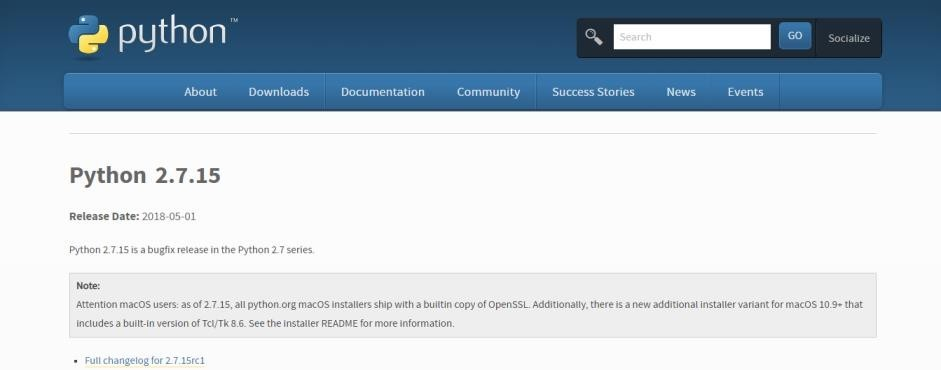
\includegraphics[width=0.70\textwidth]{figures/8/python.jpg}
	\caption{Download Softfile Python 2.7.}
	\label{fig:python}
\end{figure}

\end{enumerate}

Perintah python flask. Contoh \textit{source code} seperti pada listing \ref{lst:hello}.
\lstinputlisting[caption=Contoh kode program hello.py, label={lst:hello}]{src/8/hello.py}
 Contoh \textit{source code} main.py seperti pada listing \ref{lst:main}.
\lstinputlisting[caption=Contoh kode program main.py, label={lst:main}]{src/8/main.py}
